\documentclass{article}
\usepackage[utf8]{inputenc}
\usepackage[T1]{fontenc}
\usepackage[spanish]{babel}
\usepackage[hidelinks]{hyperref}
\usepackage{graphicx}
\usepackage{titling}
\usepackage{float}
\usepackage[text={18cm,21cm},centering]{geometry}
\usepackage{hyperref} \hypersetup{ colorlinks=true, linkcolor=blue, filecolor=magenta,
urlcolor=blue, }
\usepackage{listings}
\usepackage{xcolor}
\usepackage{booktabs}



% Definir colores adicionales si es necesario
\definecolor{gray}{rgb}{0.5, 0.5, 0.5}
\definecolor{lightgray}{rgb}{0.9, 0.9, 0.9}
\definecolor{green}{rgb}{0, 0.5, 0}
\definecolor{blue}{rgb}{0, 0, 1}
\definecolor{red}{rgb}{1, 0, 0}

\lstdefinestyle{mystyle}{
    backgroundcolor=\color{white},   
    commentstyle=\color{green},
    keywordstyle=\color{blue},
    numberstyle=\tiny\color{gray},
    stringstyle=\color{red},
    basicstyle=\ttfamily\footnotesize,
    breakatwhitespace=false,         
    breaklines=true,                 
    captionpos=b,                    
    keepspaces=true,                 
    numbers=left,                    
    numbersep=5pt,                  
    showspaces=false,                
    showstringspaces=false,
    showtabs=false,                  
    tabsize=2
}

\lstset{style=mystyle}


\begin{document}


\begin{titlepage}
    \centering
    {\bfseries\LARGE Universidad de La Habana \par}
    \vspace{1cm}
    {\scshape\Large Facultad de Matemática y Computación \par}
    \vspace{3cm}
    {\scshape\Huge Predicción de Problemas de Codeforces\par}
    \vfill
    
    {\Large Juan Carlos Espinosa Delgado C-411 \par}
    {\Large Raudel Alejandro Gómez Molina C-411 \par}
    {\Large Alex Sierra Alcalá C-411 \par}
    {\Large Yoan Rene Ramos Corrales C-412 \par}
    \vfill
    {\href{https://github.com/ARJ-Code/codeforce-tag-predictor}{Proyecto en github} \par}
\end{titlepage}

\section{Introducción}

\subsection{Motivación}

La plataforma Codeforces es una herramienta fundamental en la comunidad de programación competitiva, diseñada
para desarrollar y entrenar habilidades de resolución de problemas. Los problemas en Codeforces no solo desafían
a los competidores, sino que también proporcionan una base sólida para aprender y aplicar diversos algoritmos y
estructuras de datos. Cada problema está asociado a una serie de categorías o etiquetas que ayudan a identificar
los tipos de algoritmos y técnicas necesarias para resolverlos. Pero este proceso suele estar muy apegado a la
a la solución final del ejercicio por lo que la correcta identificación de los tags suele ser un gran reto para los
competidores.

Es válido aclarar que la automatización de este proceso no es interés de la programación competitiva, ya que en estos
escenarios lo que se busca es el razonamiento lógico de los competidores, en este contexto si pudiera ser interesante
el desarrollo de un mecanismo de generación de problemas, pero este no es el objetivo de este proyecto.

Sin embargo la experimentación con la detección de tags en escenarios controlados como este, manteniéndonos en el entorno
de que esta tarea es útil para la posterior solución del problema pudiera servir de base para proponer mecanismo de detección
de tags en problemas reales orientados al campo de la generación de algoritmos.

\subsection{Problemática}

Cada problema en la plataforma Codeforces y un problema de programación competitiva en general cuenta primeramente con
un título y una descripción en la cual se plantea el objetivo y la problemática del mismo, este segundo componente del
problema es la principal fuente de interés para la detección de tags ya que estos se encuentran explícitos en forma de
lenguaje natural en dicha descripción.

Pero además de la descripción los problemas cuentan con una restricción de tiempo y espacio de memoria donde se deben
desenvolver los algoritmos que den solución al problema (un algoritmo correcto para todos los casos de prueba
que no este dentro de los límites establecidos no es considerado como solución). Ahora bien esta restricción también
influye en los tags del algoritmo ya el conjunto de tags del problema que satisfacen estas restricciones y la descripción
del problema será subconjunto del conjunto de tags solo asociados a la descripción.

Otra característica interesante que nos pudiera aportar información sobre la naturaleza del problema es analizar el
código de una solución aceptada del problema, ya que es posible identificar los tags asociados a dicho código y por
tanto un subconjunto de los tags del problema. Es importante analizar que con este enfoque solo podemos obtener un
subconjunto de los tags ya que un mismo problema puede tener multiples soluciones y cada solución puede tener asociada
distintos tipos de tags.

Por tanto como tenemos de por medio un problema asociado a lenguaje natural y actualmente no hay ningún método asociado
medianamente eficaz asociado a este campo que no lleve Machine Learning, la propuesta de la solución descrita en este
trabajo empleará algoritmos de Machine Learning los cuales iremos introduciendo a lo largo de este trabajo.

\subsection{Objetivos Generales y Específicos}

\subsubsection{Objetivos Generales}

El objetivo general de este proyecto es desarrollar un sistema automatizado utilizando técnicas de Machine Learning para detectar y asignar etiquetas (tags) a los problemas de programación en Codeforces.


\subsubsection{Objetivos Específicos}

\begin{itemize}
    \item \textbf{Recolección y Preprocesamiento de Datos:}
          \begin{itemize}
              \item Recolectar un conjunto representativo de problemas de Codeforces, incluyendo sus descripciones, restricciones de tiempo y memoria, y etiquetas existentes.
              \item Realizar el preprocesamiento del texto de las descripciones para normalizar y limpiar los datos, facilitando su análisis.
          \end{itemize}
          
    \item \textbf{Desarrollo del Modelo de Machine Learning:}
          \begin{itemize}
              \item Investigar y seleccionar algoritmos de Machine Learning apropiados para la tarea de clasificación de texto, como KNN, Naive Bayes, y redes neuronales.
              \item Entrenar varios modelos utilizando el conjunto de datos preprocesado, ajustando hiperparámetros para optimizar el rendimiento.
          \end{itemize}
          
    \item \textbf{Evaluación del Modelo:}
          \begin{itemize}
              \item Evaluar los modelos entrenados utilizando métricas de rendimiento como precisión, recall, F1-score y exactitud.
              \item Comparar los resultados de diferentes modelos para identificar el más eficaz en la detección de etiquetas.
              \item Comparar los resultados con un modelo de lenguaje (en este caso se usará Chat-GPT 3.5).
          \end{itemize}
          
    \item \textbf{Implementación y Prueba:}
          \begin{itemize}
              \item Implementar el modelo seleccionado en un entorno de prueba para evaluar su rendimiento en condiciones reales.
              \item Realizar pruebas adicionales para validar la consistencia y robustez del sistema en la asignación de etiquetas.
          \end{itemize}
          
    \item \textbf{Documentación y Propuesta de Mejora:}
          \begin{itemize}
              \item Documentar el proceso completo de desarrollo, incluyendo la recolección de datos, preprocesamiento, desarrollo del modelo, evaluación e implementación.
              \item Proponer mejoras y futuras líneas de investigación basadas en los resultados obtenidos y las limitaciones encontradas durante el desarrollo del proyecto.
          \end{itemize}
\end{itemize}

\subsubsection{Hipótesis}

\begin{itemize}
    \item \textbf{Hipótesis Principal:} Un modelo de Machine Learning bien entrenado puede detectar y asignar etiquetas (tags) a los problemas de programación de Codeforces con una precisión comparable a la de un humano experto.
    \item \textbf{Hipótesis Secundarias:}
          \begin{itemize}
              \item Los algoritmos de clasificación de texto basados en redes neuronales (como LSTM o Transformers) ofrecerán un mejor rendimiento en la detección de etiquetas en comparación con algoritmos más tradicionales como Naive Bayes o KNN.
              \item El análisis y utilización de las restricciones de tiempo y memoria, así como del código de soluciones aceptadas, pueden mejorar significativamente la precisión del modelo en la asignación de etiquetas.
          \end{itemize}
\end{itemize}

\subsubsection{Preguntas Científicas}

\begin{itemize}
    \item ¿Qué algoritmos de Machine Learning son más efectivos para la tarea de detección de etiquetas en problemas de programación competitiva?
    \item ¿Cómo influye la calidad y cantidad de los datos de entrenamiento en el rendimiento del modelo?
    \item ¿En qué medida las restricciones de tiempo y memoria impactan en la precisión de la detección de etiquetas?
    \item ¿Es posible mejorar la detección de etiquetas utilizando información adicional del código de soluciones aceptadas?
    \item ¿Cuáles son las principales limitaciones y desafíos al aplicar Machine Learning en la detección de etiquetas en problemas de programación competitiva?
\end{itemize}

\section{Análisis de los datos}

Como dataset usaremos un conjunto de problemas de Codeforces con su identificador, descripción, conjunto de tags, puntos y rating. 

\subsection{Exploración de datos}

Para esto primero exploramos los datos buscando filas con ausencia de datos y eliminamos datos que no son de interés para
nuestro problema. 

En este caso hemos identificado que las columnas asociadas a los puntos y el rating cuentan con valores neuronales
y no representan interés para nuestro problema por lo que hemos decidido eliminarlas.

Luego analizamos el contenido de la descripción de los problemas y identificamos el idioma de las mismas ya que esta
información puede ser útil para el futuro análisis empleando modelos de lenguaje.

\subsubsection{Información recopilada sobre los datos}

\begin{itemize}
    \item Distribución de la longitud del texto de los Problemas
          \begin{center}
              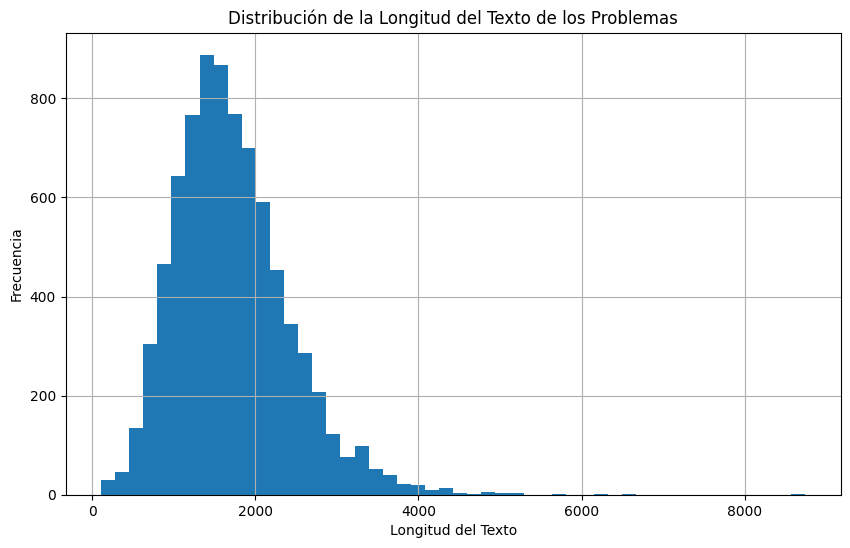
\includegraphics[scale=0.8]{imgs/len_description.png}
          \end{center}
          \newpage          
    \item Frecuencia de las etiquetas más comunes
          \begin{center}
              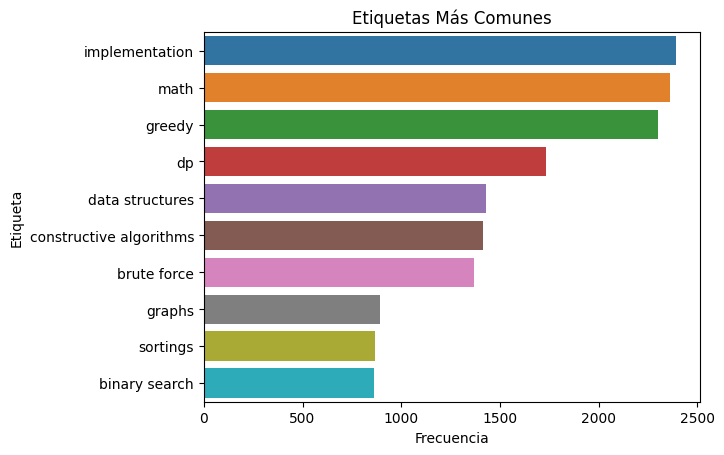
\includegraphics[scale=0.8]{imgs/common_tags_count.png}
          \end{center}
    \item Distribución de idiomas
          \begin{center}
              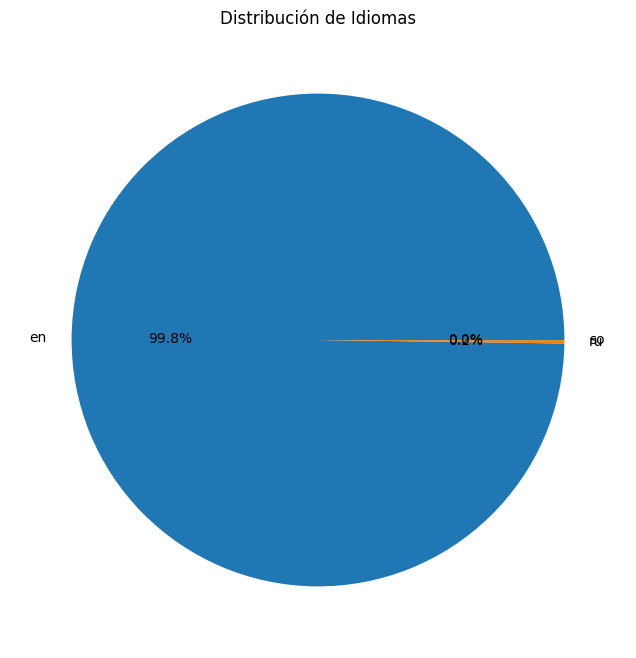
\includegraphics[scale=0.6]{imgs/langs_dist.png}
          \end{center}
          \newpage
          
    \item Nube de palabras asociada a la descripción de los problemas
          \begin{center}
              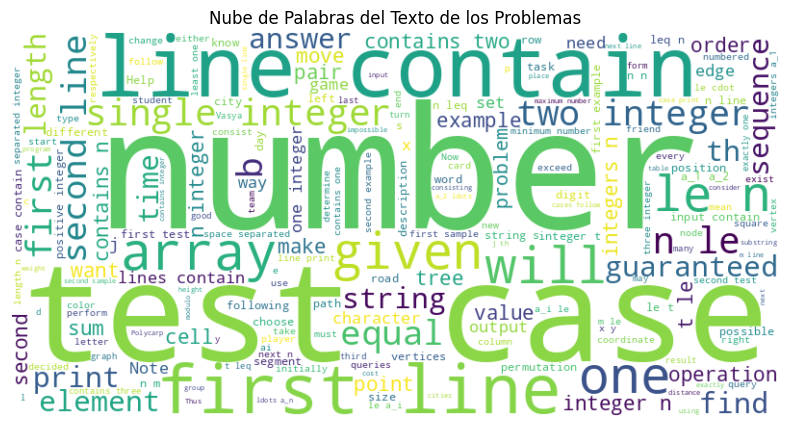
\includegraphics[scale=0.55]{imgs/wordcloud.png}
          \end{center}
    \item Matriz de correlación de las etiquetas
          \begin{center}
              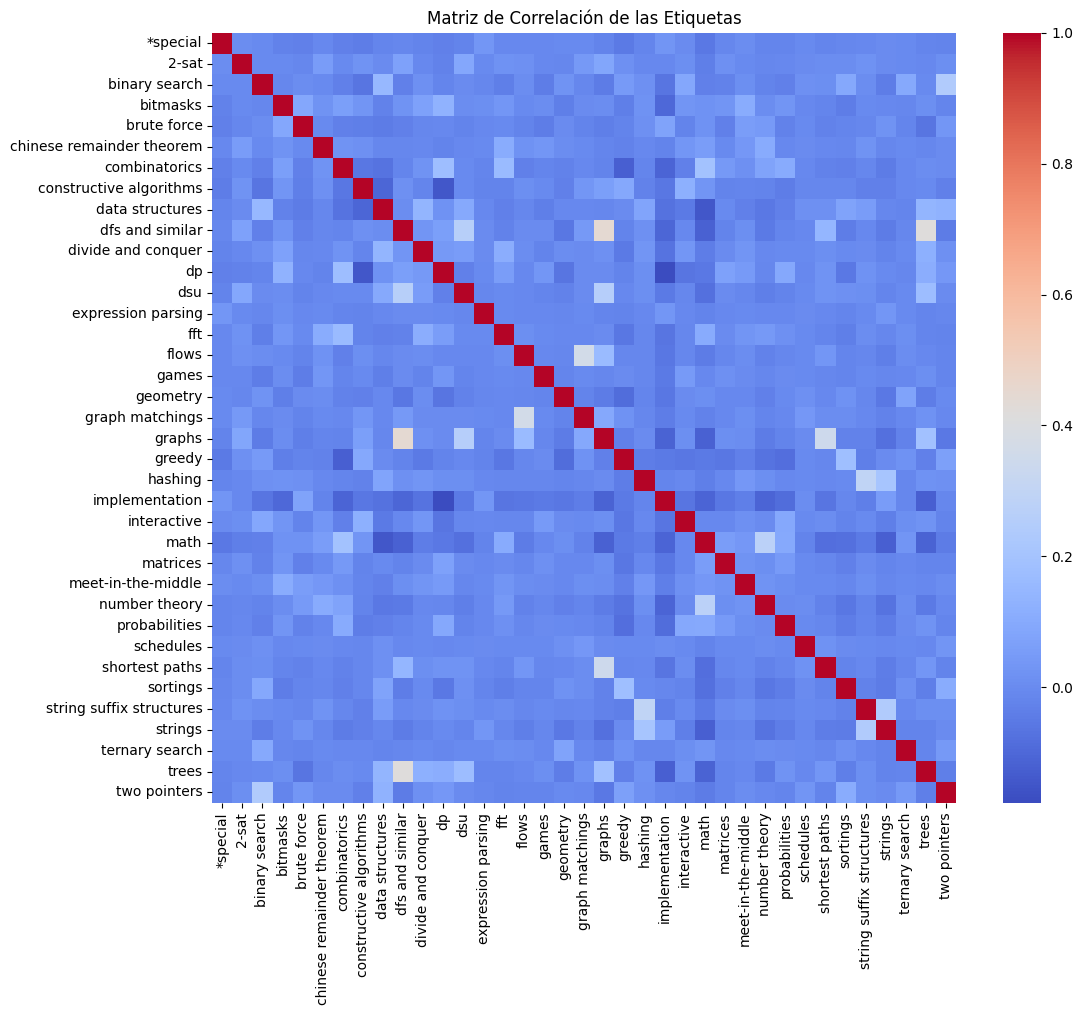
\includegraphics[scale=0.5]{imgs/correlation_matrix.png}
          \end{center}
\end{itemize}

\subsection{Preprocesamiento de datos}

\section{Estado del arte / Preliminares}

Debe incluir una revisión de la literatura sobre el problema y problemas similares.

\section{Propuestas de solución}
	\begin{itemize}
    		\item Clasificación Multietiqueta con TF-IDF y Naive Bayes
	\end{itemize}

\section{Experimentación y resultados}

\subsection{Clasificación Multietiqueta con TF-IDF y Naive Bayes}
		\subsubsection{Introducción}
La clasificación multietiqueta es una variante de la clasificación en la que cada instancia puede pertenecer a múltiples clases simultáneamente. En este estudio, utilizamos la vectorización TF-IDF para la extracción de características y un clasificador Naive Bayes para la clasificación. El objetivo principal es evaluar el rendimiento del modelo en varias métricas de evaluación.
		\subsubsection{Metodología}
			\begin{itemize}
    \item Preprocesamiento de Datos
\end{itemize}
El conjunto de datos preprocesado pasa a utilizar la vectorización TF-IDF para convertir los datos de texto en características numéricas. Las etiquetas se binarizaron utilizando \texttt{MultiLabelBinarizer} para adaptarse a la naturaleza multietiqueta del problema.

\begin{itemize}
    \item Entrenamiento del Modelo
\end{itemize}
La clasificación se realizó utilizando un clasificador Naive Bayes dentro de un marco One-vs-Rest. El conjunto de datos se dividió en conjuntos de entrenamiento y prueba utilizando una división 80-20. Una vez el modelo predecía habían problemas a los cuales no se les
asignaba ninguna etiqueta, cosa que no sucede en el codeforces, por lo cual se le hace asignar a dichos problemas la eqtiqueta más probable, garantizando así que todo problema contenga al menos una etiqueta.
\begin{verbatim}
vectorizer = TfidfVectorizer()
X = vectorizer.fit_transform(text_data)
mlb = MultiLabelBinarizer()
y = mlb.fit_transform(labels)

X_train, X_test, y_train, y_test = train_test_split(X, y, test_size=0.2, random_state=42)

clf = OneVsRestClassifier(MultinomialNB())
clf.fit(X_train, y_train)
y_pred = clf.predict(X_test)
\end{verbatim}

		\subsubsection{Resultados}
		\begin{itemize}
    			\item Informe de Clasificación
		\end{itemize}
\begin{verbatim}
classification_report(y_test, y_pred, target_names=mlb.classes_)
\end{verbatim}

\begin{verbatim}
                        precision    recall  f1-score   support

            bruteforce       0.20      0.02      0.03        61
constructivealgorithms       0.50      0.01      0.03        73
        datastructures       1.00      0.04      0.08        49
         dfsandsimilar       0.00      0.00      0.00         4
                    dp       0.00      0.00      0.00        50
              geometry       1.00      0.18      0.30        17
                greedy       0.52      0.41      0.46       111
        implementation       0.52      0.69      0.59       142
                  math       0.63      0.29      0.39       101
               strings       0.83      0.37      0.51        27

             micro avg       0.55      0.30      0.39       635
             macro avg       0.52      0.20      0.24       635
          weighted avg       0.52      0.30      0.32       635
           samples avg       0.54      0.33      0.39       635


\end{verbatim}

\begin{itemize}
    	\item Accuracy
\end{itemize}
\begin{verbatim}
Overall Accuracy: 14.46\%
\end{verbatim}
		
\begin{itemize}
    	\item Matriz de Confusión
\end{itemize}		
Se tiene un {\href{https://github.com/ARJ-Code/codeforce-tag-predictor/blob/main/src/naive\%20bayes\%20model/naive-bayes-model.ipynb}{jupyter interactivo}} en el que se puede consultar la matriz de confusión para cada etiqueta 
\newpage
\begin{itemize}
    	\item Precision ,F1-Score ,Recall y Support para cada etiqueta
\end{itemize}
\begin{figure}[H]
    \centering
    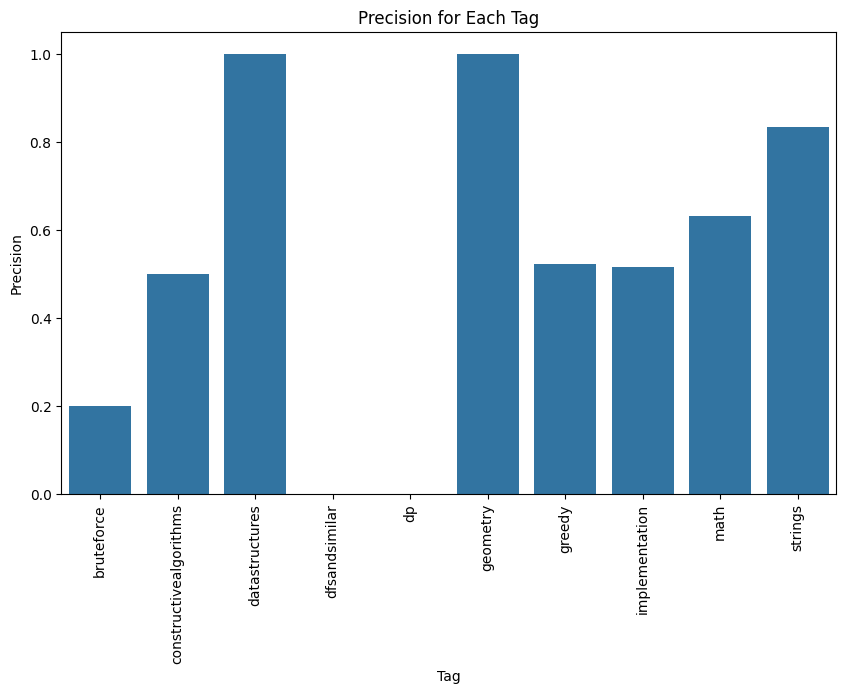
\includegraphics[width=0.8\textwidth]{imgs/precisonnb.png}
    \caption{Precision}
    \label{fig:p}
\end{figure}
\newpage
\begin{figure}[H]
    \centering
    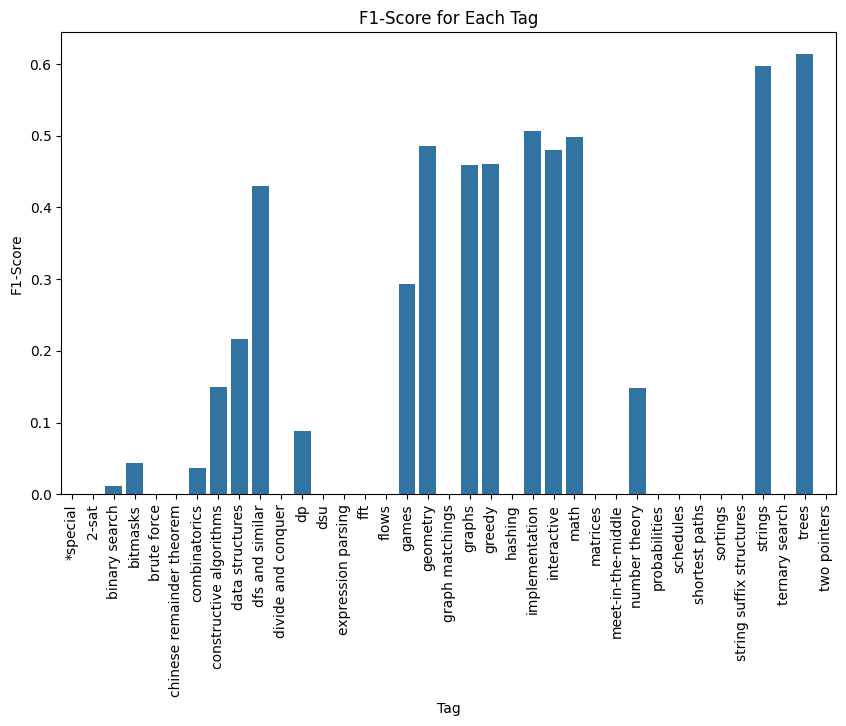
\includegraphics[width=0.8\textwidth]{imgs/f1nb.png}
    \caption{F1-Score}
    \label{fig:f1}
\end{figure}
\begin{figure}[H]
    \centering
    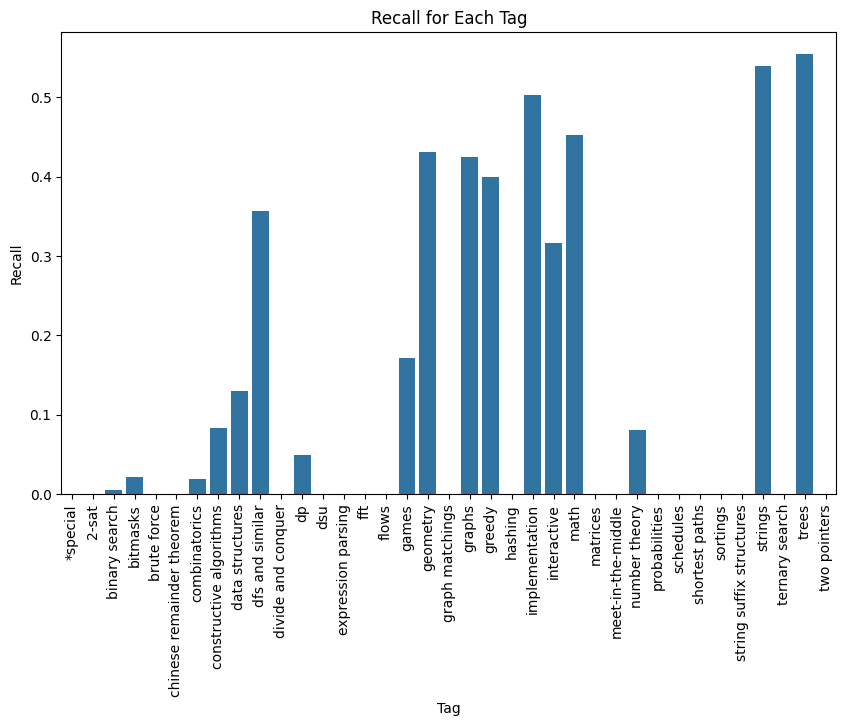
\includegraphics[width=0.8\textwidth]{imgs/recallnb.png}
    \caption{Recall}
    \label{fig:r}
\end{figure}
\begin{figure}[H]
    \centering
    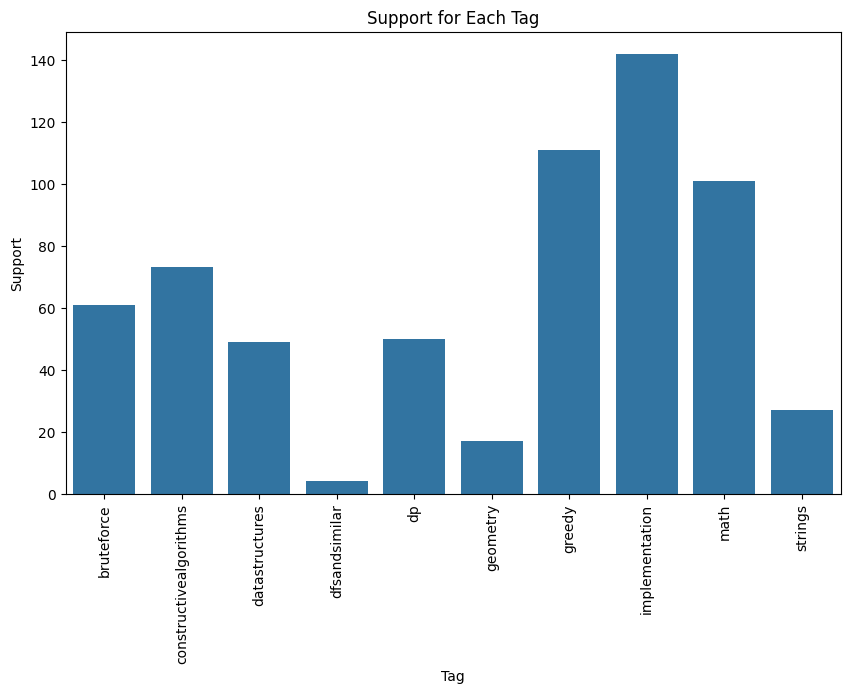
\includegraphics[width=0.8\textwidth]{imgs/supportnb.png}
    \caption{Support}
    \label{fig:s}
\end{figure}

\subsection{Chat GPT}

Para analizar que tan bien se comportaba Chat GPT 3.5, prediciendo los tags de Codeforces, usamos prompt engineering
con un preprocesamiento sobre los problemas:

\begin{lstlisting}[language=Python, caption=Prompt para tagear los problemas]
def prompt(description):
    all_tags_str = ', '.join(all_tags)
    return f'Give this set of {all_tags_str} tags and this problem ${description}, give me the set of problem tags in the following format: greedy, implementation, dp'
\end{lstlisting}

\begin{tabular}{llrr}
    \toprule
    {} & Metric        & ChatGPT & Naive Bayes \\
    \midrule
    0  & Accuracy      & 0.020000 & 0.146000 \\
    1  & F1 (macro)    & 0.002431  & 0.240000 \\
    2  & F1 (micro)    & 0.020000 & 0.390000 \\
    3  & F1 (weighted) & 0.017556 & 0.320000 \\
    4  & F1 (samples)  & 0.002431  & 0.390000 \\
    \bottomrule
\end{tabular}

\section{Discusión de los resultados}
Debe incluir la repercusión ética de las soluciones.

\section{Conclusiones y trabajo futuro}


\end{document}